\section{Pipeline Template}
Our approach integrates data protection and data management into the service pipeline using annotations.
To this aim, we extend the service pipeline in \cref{def:pipeline} with: \emph{i)} data protection annotations expressing transformations on data to enforce data protection requirements, \emph{ii)} functional annotations expressing data manipulations carried out during services execution.
These annotations permit to implement an advanced data lineage, tracking the entire data lifecycle by monitoring changes arising from functional service execution and data protection requirements.

In the following, we first introduce the annotated service pipeline, called pipeline template in Section \ref{sec:templatedefinition}. We then present functional annotations (Section \ref{sec:funcannotation}) and data protection annotations (Section \ref{sec:nonfuncannotation}). We finally provide an example of a pipeline template (Section \ref{sec:example}).


\subsection{Pipeline Template Definition}\label{sec:templatedefinition}
Given the service pipeline in Definition~\ref{def:pipeline}, we use annotations to express data protection requirements to be enforced on data and functional requirements on services to be integrated in the pipeline. Each service vertex in the service pipeline is labeled with two mapping functions forming a pipeline template:
\begin{enumerate*}[label=\roman*)]
  \item a labeling function \myLambda:\V$\rightarrow$\P{} that associates a set of data protection requirements, in the form of policies $p_i\in$\P{}, with each vertex \vi{i}$\in$\V$_S$;
  \item a labeling function \myGamma:\V$\rightarrow$\F{} that associates a functional service description $F_i\in\F{}$ with each vertex \vi{i}$\in$\V$_S$.
\end{enumerate*}
%The policies will be intended to guide the enforcement of data protection while the data transformation function will characterize the functional aspect of each vertex.

The template is formally defined as follows.

\begin{definition}[Pipeline Template] \label{def:template}
  Given a service pipeline G(\V,\E), a pipeline template $G^{\myLambda,\myGamma}$(V,E,\myLambda,\myGamma) is a direct acyclic graph with two labeling functions:
  \begin{enumerate}[label=\roman*)]
    \item \myLambda that assigns a label \myLambda(\vi{i}), corresponding to a policy $p_i$ to be satisfied by service $s_i$ represented by \vi{i}, for each vertex $\vi{i}\in\V$;
    \item \myGamma that assigns a label \myGamma(\vi{i}), corresponding to the functional description $F_i$ of service $s_i$ represented by \vi{i}, for each vertex $\vi{i}\in\V$.
  \end{enumerate}
\end{definition}

We note that, at this stage, the template is not yet linked to any services, nor it is possible to determine the policy modeling the specific data protection requirements.
%We also note that functional description $F_i$ includes the specific data transformation triggered as the result of a service execution.
An example of pipeline template is depicted in \cref{fig:service_composition_template}

%The next sections better explain the functional and non-functional transformation functions.
\begin{figure}[ht!]
  \centering
  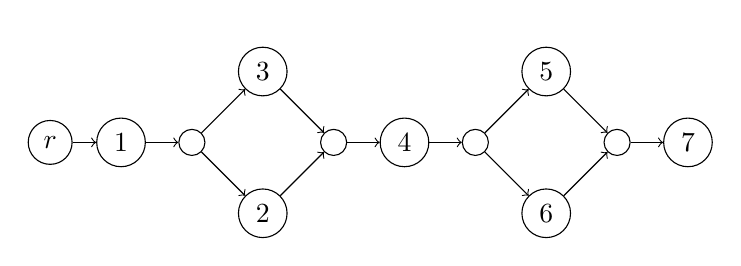
\begin{tikzpicture}[scale=0.9]
    % Nodes
    \node[draw, circle] (node1) at (0,0) {$\s{r}$};
    \node[draw, circle] (node2) at (1,0) {$\s{1}$};
    \node[draw, circle] (node3) at (2,0) {$\timesOperator$};
    \node[draw, circle] (node4) at (3,-1) {$\s{2}$};
    \node[draw, circle] (node5) at (3,1) {$\s{3}$};
    \node[draw, circle] (node6) at (4,0) {$\timesOperator$};
    \node[draw, circle] (node65) at (5,0) {$\s{4}$};
    \node[draw, circle] (node7) at (6,0) {$\plusOperator$};
    \node[draw, circle] (node8) at (7,1) {$\s{5}$};
    \node[draw, circle] (node9) at (7,-1) {$\s{6}$};
    \node[draw, circle] (node10) at (8,0) {$\plusOperator$};
    \node[draw, circle] (node11) at (9,0) {$\s{7}$};
    % Text on top
    \node[above] at (node1.north)  {$\templateChartAnnotation$};
    \node[above] at (node2.north)  {$\templateChartAnnotation$};
    \node[above] at (node3.north)  {                 };
    \node[above] at (node4.north)  {$\templateChartAnnotation$};
    \node[above] at (node5.north)  {$\templateChartAnnotation$};
    \node[above] at (node65.north) {$\templateChartAnnotation$};
    \node[above] at (node8.north)  {$\templateChartAnnotation$};
    \node[above] at (node9.north)  {$\templateChartAnnotation$};
    \node[above] at (node11.north) {$\templateChartAnnotation$};
    % Connection
    \draw[->] (node1) -- (node2);
    \draw[->] (node2) -- (node3);
    \draw[->] (node3) -- (node4);
    \draw[->] (node3) -- (node5);
    \draw[->] (node5) -- (node6);
    \draw[->] (node4) -- (node6);
    \draw[->] (node6) -- (node65);
    \draw[->] (node65) -- (node7);
    \draw[->] (node7) -- (node8);
    \draw[->] (node7) -- (node9);
    \draw[->] (node8) -- (node10);
    \draw[->] (node9) -- (node10);
    \draw[->] (node10) -- (node11);
  \end{tikzpicture}
  \caption{Pipeline Template}
  \label{fig:service_composition_template}
\end{figure}

\begin{figure}[ht!]
  \centering
  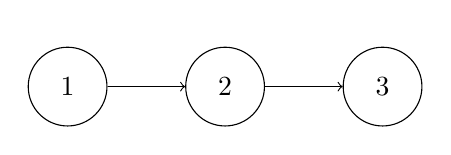
\begin{tikzpicture}
    % Nodes
    \node[draw, circle,minimum size=1cm] (node1) at (0,0) {$\s{1}$};
    \node[draw, circle,minimum size=1cm] (node2) at (2,0) {$\s{2}$};
    \node[draw, circle,minimum size=1cm] (node3) at (4,0) {$\s{3}$};

    \node[above] at (node1.north)  {$\templateChartAnnotation$};
    \node[above] at (node2.north)  {$\templateChartAnnotation$};
    \node[above] at (node3.north)  {$\templateChartAnnotation$};

    % Connection
    \draw[->] (node1) -- (node2);
    \draw[->] (node2) -- (node3);

  \end{tikzpicture}
  \caption{Pipeline Template Example}
  \label{fig:temp}
\end{figure}

\subsection{Data Protection Annotation \myLambda}\label{sec:nonfuncannotation}
Data Protection Annotation \myLambda\ expresses data protection requirements in the form of access control policies. We consider an attribute-based access control model that offers flexible fine-grained authorization and adapts its standard key components to address the unique characteristics of a big data environment. Access requirements are expressed in the form of policy conditions that are defined as follows.

\begin{definition}[Policy Condition]\label{def:policy_cond}
  A \emph{Policy Condition} is a Boolean expression of the form $($\emph{attr\_name} op \emph{attr\_value}$)$, with op$\in$\{$<$,$>$,$=$,$\neq$,$\leq$,$\geq$\}, \emph{attr\_name} an attribute label, and \emph{attr\_value} the corresponding attribute value.
\end{definition}

An access control policy then specifies who (\emph{subject}) can access what (\emph{object}) with action (\emph{action}), in a specific context (\emph{environment}) and under specific obligations (\emph{data transformation}), as formally defined below. 

\begin{definition}[Policy]\label{def:policy_rule}
  A {\it policy P} is 5-uple $<$\textit{subj}, \textit{obj}, \textit{action}, \textit{env}, \textit{\TP}$>$, where:
  \begin{description}
    \item Subject \textit{subj} defines a service $s_i$ issuing an access request to perform an action on an object. It is of the form $<$\emph{id}, \emph{PC}$>$, where \emph{id} defines a class of services (e.g., classifier), and \emph{PC} is a set of \emph{Policy Conditions} on the subject, as defined in Definition \ref{def:policy_cond}. For instance, $<$\emph{service},\{(classifier $=$ "SVM")\}$>$ refers to a service providing a SVM classifier. We note that \textit{subj} can also specify conditions on the service owner, such as, $<$\emph{service},\{(owner\_location $=$ "EU")\}$>$

    \item Object \textit{obj} defines any data whose access is governed by the policy. It is of the form $<$\emph{type}, \emph{PC}$>$, where: \emph{type} defines the type of object, such as a file (e.g., a video, text file, image, etc.), a SQL or noSQL database, a table, a column, a row, or a cell of a table, and \emph{PC} is a set of \emph{Policy Conditions} defined on the object's attributes. For instance, $<$\emph{dataset},\{(region $=$ CT)\}$>$ refers to a dataset whose region is Connecticut.

    \item Action \textit{action} defines any operations that can be performed within a big data environment, from traditional atomic operations on databases (e.g., CRUD operations varying depending on the data model) to coarser operations, such as an Apache Spark Direct Acyclic Graph (DAG), Hadoop MapReduce, an analytics function call, or an analytics pipeline.

    \item Environment \textit{env} defines a set of conditions on contextual attributes, such as time of the day, location, IP address, risk level, weather condition, holiday/workday, emergency. It is a set \emph{PC} of \emph{Policy Conditions} as defined in Definition \ref{def:policy_cond}. For instance, $<$\emph{env},\{(time $=$ "night")\}$>$ refers to a policy that is applicable only at night.

    \item Data Transformation \textit{\TP} defines a set of security and privacy-aware transformations on \textit{obj}, which must be enforced before any access to data. Transformations focus on data protection, as well as compliance to regulations and standards, in addition to simple format conversions. 
  \end{description}
\end{definition}

An access control policy $P$ annotated in a pipeline template $G^{\myLambda,\myGamma}$ is used to filter out those candidate services $s$ that do not match data protection requirements. Specifically, a policy $P_i$ is evaluated to verify whether a candidate service $s_j$ for vertex \vi{i} is compatible with data protection requirements in $P_i$ (\myLambda(\vi{i})). Policy evaluation matches the profile of candidate service $s_j$ with the policy conditions in $P_i$. If the credentials and attributes in the candidate service profile fails to meet the policy conditions, the service is discarded, otherwise it is added to the set of compatible service, which is used in Section~\ref{} to generate the pipeline instance $G'$. No policy enforcement is done at this stage.

\subsection{Functional Annotations \myGamma}\label{sec:funcannotation}
A proper data management approach must track functional data manipulations across the entire pipeline execution, defining the functional requirements of each service operating on data.
To this aim, each vertex \vi{i}$\in$\V$_S$ is annotated with a label \myGamma(\vi{i}), corresponding to the functional description $F_i$ of the service $s_i$ represented by \vi{i}.
$F_i$ describes the functional requirements on the corresponding service $s_i$, such as API, inputs, expected outputs.
%The latter is modeled as a functional transformation function \TF\ that is applied to the data when executing service $s_i$. \TF\ has a twofold role:
%\begin{enumerate}[label=\roman*)]
%  \item it contains the functional requirements that the service must satisfy, in terms of expected input, expected output, prototype and other functional aspects.
%  \item
It also specifies the specific data transformation function \TF{}, triggered as the result of a service execution. %applied to the data when executing service $s_i$.

This function can be classified according to four types.
\begin{enumerate*}[label=\roman*)]
  \item Function \TF{\epsilon}, an empty function that applies no transformation or processing on the data.
  \item Function \TF{a}, an additive function that expands the amount of data received, for example, by integrating data from other sources.
  \item Function \TF{t}, a transformation function that transforms some records in the dataset without altering the domain.
  \item Function \TF{d} (out of the scope of this work), a transformation function that changes the domain of the data by applying, for instance, PCA or K-means.
\end{enumerate*}
%A transformation function can be classified according to four types.
% \begin{enumerate*}[label=\roman*)]
%   \item Function \F{e}, an empty function that applies no transformation or processing on the data.
%   \item Function \F{a}, an additive function that expands the amount of data received, for example, by integrating data from other sources.
%   \item Function \F{t}, a transformation function that transforms some records in the dataset without altering the domain.
%   \item Function \F{d}, a transformation function that changes the domain of the data by applying, for instance, PCA or K-means (out of the scope of this work).
% \end{enumerate*}

\subsection{Example}\label{sec:example}
As an example, let us consider a pipeline template $G^{\myLambda,\myGamma}$ with three vertices, as depicted in \cref{fig:service_composition_example}.
It includes three key stages in our reference scenario: data anonymization (\vi{1}), data enrichment (\vi{2}), and data aggregation (\vi{3}), each stage with its policy $p$ and functional description \F.

%\begin{enumerate*}[label=n\arabic*)]
%  \item
The first vertex (\vi{1}) is responsible for data anonymization.
It specifies an anonymization policy ($\myLambda(v_1)$) to protect sensitive information, such as personally identifiable information (PII) in the dataset.
The transformation function \TF{1} in $\myGamma(v_1)$ is an empty function \TF{a}, as no functional transformation is required for anonymization.
%   \item

The second vertex (\vi{2}) focuses on data enrichment, where additional information from the states of New York and New Hampshire is integrated into the dataset.
It requires a data enrichment policy ($\myLambda(v_2)$) to ensure that the added data is relevant and compliant with privacy regulations.
The transformation function \TF{2} in $\myGamma(v_2$) is an additive function \TF{a}, which merges and integrates the external data with the existing dataset.
  %  \item

  The third vertex (\vi{3}) is responsible for aggregating data, including statistical measures like averages, medians, and some more statistics.
  It follows an aggregation policy ($\myLambda(v_3)$) to define how the aggregation should be performed, and ensure compliance with privacy and security regulations.
  The transformation function \TF{3} in $\myGamma(v_3)$ is a transformation function \TF{t}, which computes the required statistics and aggregates the data.
  %\end{enumerate*}

  \begin{figure}[ht!]
    \centering
    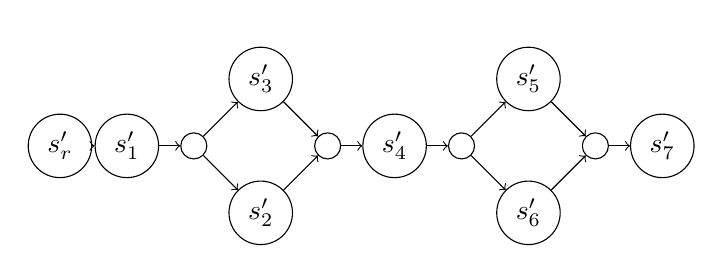
\begin{tikzpicture}[scale=0.85]
      \node[draw, circle] (node1) at (0,0) {$s^\prime_r$};
      \node[draw, circle] (node2) at (1,0) {$s^\prime_1$};
      \node[draw, circle] (node3) at (2,0) {$\timesOperator$};
      \node[draw, circle] (node4) at (3,-1) {$s^\prime_2$};
      \node[draw, circle] (node5) at (3,1) {$s^\prime_3$};
      \node[draw, circle] (node6) at (4,0) {$\timesOperator$};
      \node[draw, circle] (node65) at (5,0) {$s^\prime_4$};
      \node[draw, circle] (node7) at (6,0) {$\plusOperator$};
      \node[draw, circle] (node8) at (7,1) {$s^\prime_5$};
      \node[draw, circle] (node9) at (7,-1) {$s^\prime_6$};
      \node[draw, circle] (node10) at (8,0) {$\plusOperator$};
      \node[draw, circle] (node11) at (9,0) {$s^\prime_7$};
      % Text on top
      \node[above] at (node1.north) { \footnotesize$\instanceChartAnnotation$};
      \node[above] at (node2.north) { \footnotesize$\instanceChartAnnotation$};
      \node[above] at (node3.north) {};
      \node[above] at (node4.north) { \footnotesize$\instanceChartAnnotation$};
      \node[above] at (node5.north) { \footnotesize$\instanceChartAnnotation$};
      \node[above] at (node65.north) { \footnotesize$\instanceChartAnnotation$};
      \node[above] at (node8.north) { \footnotesize$\instanceChartAnnotation$};
      \node[above] at (node9.north) { \footnotesize$\instanceChartAnnotation$};
      \node[above] at (node11.north) { \footnotesize$\instanceChartAnnotation$};
      % Connection
      \draw[->] (node1) -- (node2);
      \draw[->] (node2) -- (node3);
      \draw[->] (node3) -- (node4);
      \draw[->] (node3) -- (node5);
      \draw[->] (node5) -- (node6);
      \draw[->] (node4) -- (node6);
      \draw[->] (node6) -- (node65);
      \draw[->] (node65) -- (node7);
      \draw[->] (node7) -- (node8);
      \draw[->] (node7) -- (node9);
      \draw[->] (node8) -- (node10);
      \draw[->] (node9) -- (node10);
      \draw[->] (node10) -- (node11);
    \end{tikzpicture}
    \caption{Service composition instance}
    \label{fig:service_composition_instance}
  \end{figure}

  \section{Pipeline Instance}
  % \subsection{Instance}
  % \hl{ANCHE QUA COME PER IL TEMPLATE PROVEREI A ESSERE UN POCO PIU' FORMALE. GUARDA IL PAPER CHE TI HO PASSATO.}
  We define a \pipeline instantiation technique as a function that takes as input a \pipelineTemplate \tChartFunction and a set $S'$ of compatible services, one for each vertex \vi{i}$\in$\V, and returns as output a \pipelineInstance \iChartFunction. We recall that compatible services $S'_i$ are candidate services satisfying data protection annotations \myLambda(\vi{i}), for each \vi{i}$\in$$\V_S$.
  In \iChartFunction, every invocations $\vi{i}$$\in$\V$_S$ contains a service instance, and every branching $v\in\Vplus\bigcup\Vtimes$ is maintained as it is. We formally define our \pipelineInstance as follows.

  \begin{definition}[Pipeline Instance]\label{def:instance}
    Let \tChartFunction be a pipeline template, a pipeline Instance $\iChartFunction$ is a directed acyclic graph where:
    \begin{enumerate*}[label=\roman*)]
      \item $s_r=s'_r$,
      \item for each vertex $\vi{}\in\V_{\timesOperator}\cup\V_{\plusOperator}$ it exists a corresponding vertex $\vii{}\in\Vp_{\timesOperator}\cup\Vp_{\plusOperator}$,
      \item for each $\vi{i}\in\V_S$ annotated with policy \P{i} it exists a corresponding \vii{i}$\in$ \Vp$_S$ instantiated with a real service $s'_i$,
    \end{enumerate*}
    and such that the following conditions hold:
    \begin{enumerate}[label=\arabic*)]
      \item $s'_i$ satisfies data protection annotation \myLambda(\vi{i}) in \tChartFunction.
      \item $s'_i$ satisfies functional annotation \myGamma(\vi{i}) in \tChartFunction.
    \end{enumerate}
  \end{definition}

  Condition 1 is needed to preserve the process functionality, as it simply states that each service $s'_i$ must satisfy the functional requirements $F_i$ of the corresponding vertex \vi{i} in the \pipelineTemplate.
  Condition 2 states that each service $s'_i$ must satisfy the policy requirements \P{i} of the corresponding vertex \vi{i} in the \pipelineTemplate.
  We assume that Condition 1 is satisfied for all candidate services and we therefore concentrate on Condition 2 in the following.

  % Le considerazioni che seguono partono dall'assunto che  T sia uguale a T_p U T_f senza lack of generality

  The \pipelineInstance  is generated by traversing the \pipelineTemplate with a breadth-first search algorithm, starting from the root vertex \vi{r}.
  Then for each vertex \vi{i} in the pipeline template, the corresponding vertex \vii{i}$\in$\Vp\ is generated.
  Finally, for each vertex \vii{i}$\in$\Vp, a two-step selection approach is applied as follows.
  \begin{itemize}

    \item \textit{Filtering Algorithm} -- As already discussed in Section~\ref{sec:templatedefinition}, filtering algorithm retrieves a set of candidate services and match them one-by-one against data protection requirements \myLambda(\vi{i}). In particular, the profile of each candidate service \si{j} is matched against policy \P{i} corresponding to \myLambda(\vi{i}). Filtering algorithm returns as output the set of compatible services that match the policy. 
    
    Formally, let us consider a set $S^c$ of candidate services \si{j}, each one annotated with a profile. The filtering algorithm is executed for each \si{j}; it is successful if \si{j}'s profile satisfies \myLambda(\vi{i}) as the access control policy \P{i}; otherwise, \si{j} is discarded and not considered for selection. The filtering algorithm finally returns a subset $S'\subseteq S^c$ of compatible services, which represent the possible candidates for selection.

    \item \textit{Comparison Algorithm} - Upon retrieving a set $S'$ of compatible services \si{j}, it produces a ranking of these services according to some metrics that evaluate the quality loss introduced by each service when integrated in the pipeline instance. More details about the metrics are provided in Section \ref{sec:metrics}. 
    %Formally, compatible services \si{j}$\in$S' are ranked on the basis of a scoring function. 
    The best service \si{j} is then selected and integrated in $\vii{i}\in \Vp$. There are many ways of choosing relevant metrics, we present those used in this article in Section \ref{sec:metrics}.
  \end{itemize}

  When all vertices $\vi \in V$ have been visited, G' contains a service instance $s'_i$ for each \vii{i}$\in$\Vp, and the \pipelineInstance is complete. We note that each vertex \vii{i} is annotated with a policy \P{i} according to \myLambda. When pipeline instance is triggered, before any services can be executed, policy \P{i} is evaluated and enforced. In case policy evaluation returns \emph{true}, data transformation \TP$\in$\P{i} is applied, otherwise a default transformation that delete all data is applied.

\begin{example}\label{ex:instance}

  As an example, let us consider the pipeline template \tChartFunction in \cref{sec:example}.
  It includes three key stages in our reference scenario: data anonymization (\vi{1}), data enrichment (\vi{2}), and data aggregation (\vi{3}), each stage with its policy $p$.

  The first vertex (\vi{1}) responsible for data anonymization is associated with three candidate services that satisfy the functional requirements of the first vertex, namely $s_1$, $s_2$ and $s_3$.
  Services $s_1$ and $s_2$ are annotated with a profile that satisfies the data protection requirements in \P{1}, respectively.
  The third service $s_3$ is annotated with a profile that does not satisfy the data protection requirements in \P{1}.
  The filtering algorithm then returns the set $S'=\{s_1,s_2\}$.
  The comparison algorithm is finally applied to $S'$ and returns a ranking of the services according to quality metrics, where $s_1$ is ranked first. $s_1$ is then selected and integrated in $\vii{1}\in \Vp$. 
  
  The same logic is applied to the \vi{2} and \vi{3}.

\end{example}


% \begin{figure}[H]
%   \centering

%   \begin{tikzpicture}
%     % Nodes
%     \node[draw, circle, minimum size=0.4cm, draw=gray, text opacity=0.5] (node11) at (0,1.2) {Sx};
%     \node[draw, circle, minimum size=1cm] (node1) at (0,0) {S1};
%     \node[draw, circle, minimum size=0.4cm, draw=gray, text opacity=0.5] (node10) at (0,-1.2) {Sy};

%     \node[draw, circle, minimum size=0.4cm, draw=gray, text opacity=0.5] (node22) at (2,1.2) {Sx};
%     \node[draw, circle, minimum size=1cm] (node2) at (2,0) {S2};
%     \node[draw, circle, minimum size=0.4cm, draw=gray, text opacity=0.5] (node21) at (2,-1.2) {Sy};

%     \node[draw, circle, minimum size=1cm] (node3) at (4,0) {$\timesOperator$};

%     \node[draw, circle, minimum size=0.4cm, draw=gray, text opacity=0.5] (node42) at (5,-1.5) {Sx};
%     \node[draw, circle, minimum size=1cm] (node4) at (6,-1.5) {S3};
%     \node[draw, circle, minimum size=0.4cm, draw=gray, text opacity=0.5] (node41) at (7,-1.5) {Sy};

%     \node[draw, circle, minimum size=1cm] (node5) at (6,1.5) {S4};
%     \node[draw, circle, minimum size=0.4cm, draw=gray, text opacity=0.5] (node51) at (5,1.5) {Sx};
%     \node[draw, circle, minimum size=0.4cm, draw=gray, text opacity=0.5] (node52) at (7,1.5) {Sy};
%     % Connection
%     \draw[->] (node1) -- (node2);
%     \draw[->] (node2) -- (node3);
%     \draw[->] (node3) -- (node4);
%     \draw[->] (node3) -- (node5);
%   \end{tikzpicture}
%   \caption{Service composition instance}
%   \label{fig:service_composition_instance}
% \end{figure}
% \[ \forall S \in \mathrm{S}_{C}  \exists  \iChartFunction(S) = \mathrm{S}_{1} \]


\begin{figure}
  \centering
  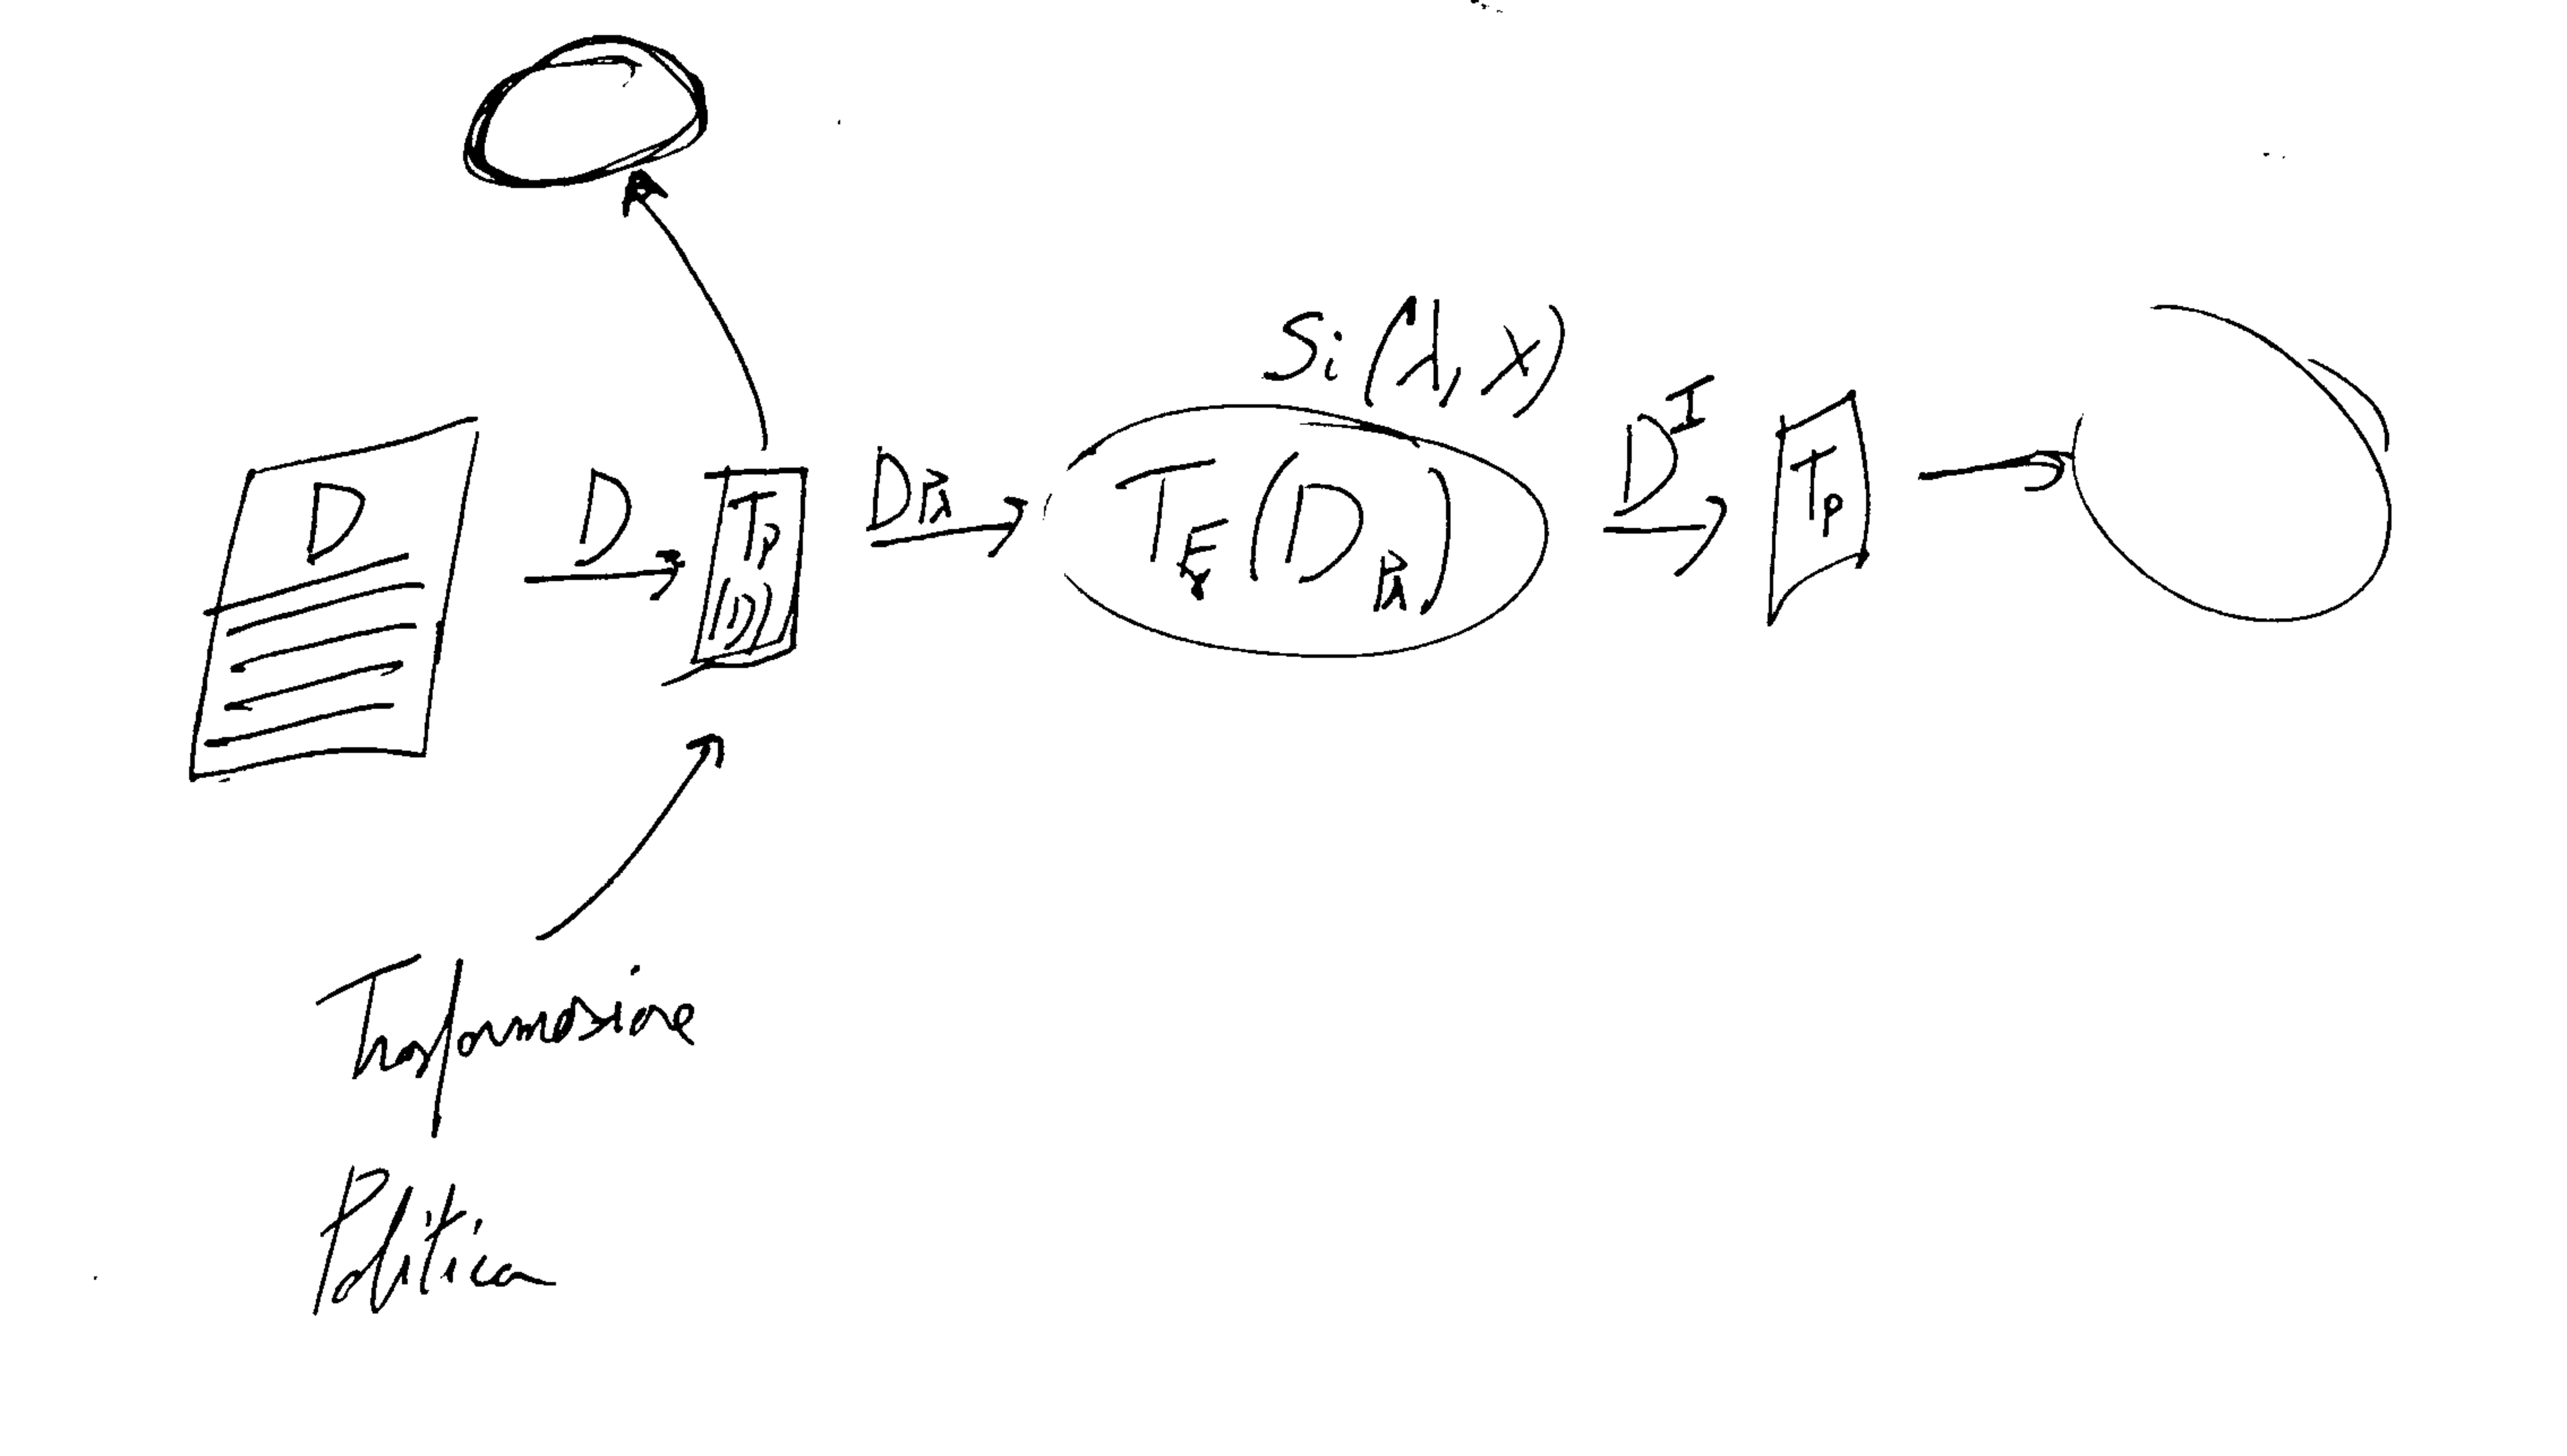
\includegraphics[width=\columnwidth]{serviceDetail.pdf}
  \caption{Service Detail}
  \label{fig:service_detail}reinstall remote-ssh
\end{figure}
